\documentclass[a4paper,12pt]{article}

\usepackage[margin=1in]{geometry}
\usepackage{graphicx}
\usepackage{float}
\usepackage{listings}
\usepackage{color}
\usepackage{subcaption}
\usepackage{url}
\lstset{language=C++,
                basicstyle=\small \ttfamily,
                keywordstyle=\color{blue}\ttfamily,
                stringstyle=\color{red}\ttfamily,
                commentstyle=\color{green}\ttfamily,
                morecomment=[l][\color{magenta}]{\#},
                breaklines=true
}
% Keywords command
\providecommand{\keywords}[1]
{
  \small	
  \textbf{\textit{Keywords---}} #1
}

\author{Ferenc Nandor Janky}
\date{}

\title{poly::vector- a sequential container for storing polymorphic objects in C++}


\begin{document}

\maketitle

\begin{abstract}
In Object-Oriented Programming paradigm dealing with collections of polymorphic types is a recurring programming pattern. Heterogeneous collections storage can not always guarantee co-locating objects resulting in access penalties on modern CPU hardware where memory caching is utilized.
This paper describes a container that has better access performance on average when storing polymorphic objects than other C++ Standard Template Library (STL) based variants. It achieves this by enforcing locality of references structurally and by reducing the number of total allocation count when a unique ownership model is desired.

\end{abstract}
 
\keywords{cache-miss, prefetch, performance, locality of references, memory allocator, OOP}



\section{Introduction \& Motivation}

One of the most recurring patterns with the object-oriented software (OOP) design paradigm is ownership and management of ownership. In order to exploit the benefits of the design principles, the use of interface, and implementation classes are required. In the C++ language, dynamic dispatch is only applicable when a particular virtual function is called through a pointer or reference to an interface class. When pointers are involved in C++, the most frequently arising question is ownership: who owns the object, i.e.,  which part of the code will free up resources associated with an object? 

There are multiple working solutions for this problem: smart pointers for expressing unique ( \lstinline{std::unique_ptr<T>}) and shared ownership ( \lstinline{std::shared_ptr<T>}) or the  \lstinline{gsl::owner<T>} from GSL libraries for marking pointers as owners of the resource while treating all others as non-owners. While the former is an active way of having a handle object to access the desired object through and also to invoke the destructor and free up the allocated memory upon the handle object's destruction, the latter one is more like an annotation. Static analyzers can flag potential leaks and undefined behaviours related to resource management based on these annotations. 

%TODO: 1-2 sentence on OOP that leads to the following paragraph.

If the objective is to have a collection of polymorphic objects whose lifetime is associated with the containing data structure, the standard solution is to use one of the standard containers parametrized with a smart pointer of the interface type, e.g: \lstinline{std::vector<std::unique_ptr<MyInterface>>}. That solution fulfills the requirements of resource management. However, if modern CPU architecture is considered - where locality of references is the key driver of performance - it might be sub-optimal as typically, the memory layout will look like as illustrated in Figure \ref{fig:stdvecbased}.

On most modern CPU architecture that uses out-of-order execution, overall performance is mostly affected by how the CPU cache is utilized. Assuming that it is more important to ensure the locality of references than optimizing asymptotic complexity - if the problem size is below a certain threshold where the former limit dominates the performance - that locality must be enforced somehow structurally to squeeze out maximum performance from both software and hardware \cite{cache_line_aware_datastructs}. In managed languages, there is no direct control available for the application programmer to manually control allocation layout, however with such system programming language as C++, this can be addressed as well - pun intended. 

Nevertheless, such data structure does not exist in the C++ Standard Library. While the Standard Template Library (STL) is being generic enough that locality can be improved by using custom allocators, and with C++17's recent addition of \lstinline{std::pmr::monotonic_buffer_resource}, this is easier than ever. The monotonic resource's only problem is that if the assigned memory resource is exhausted, it will fall back to the upstream allocator, then the locality is not guaranteed again. Moreover, if we examine the total allocation count when using e.g: \lstinline{std::pmr::vector<unique_ptr<Interface>>} it will be still higher than expected (including the object allocation as well).
 
 The purpose of this paper is to introduce a container that is specifically tailored for the use-case as mentioned earlier without the need for custom allocators while providing locality of references structurally and also keeping the total allocation count - i.e.  when the data structure requests a new chunk of memory - at the minimum. Furthermore, this container must not be comparably worse than the standard alternative in the best-case scenario while also being significantly better in the worst-case scenario. The best-case scenario means that most allocations happen successively, and in contrast, the worst-case means when random allocations happen with random longevity. Given this data structure, the memory layout would be guaranteed to look something like as illustrated by Figure \ref{fig:polyvecbased}. The implementation and the benchmarks can be obtained from \cite{poly_vec_github}
 
 
\begin{figure}
\centering
\begin{minipage}{.5\textwidth}
    \centering
    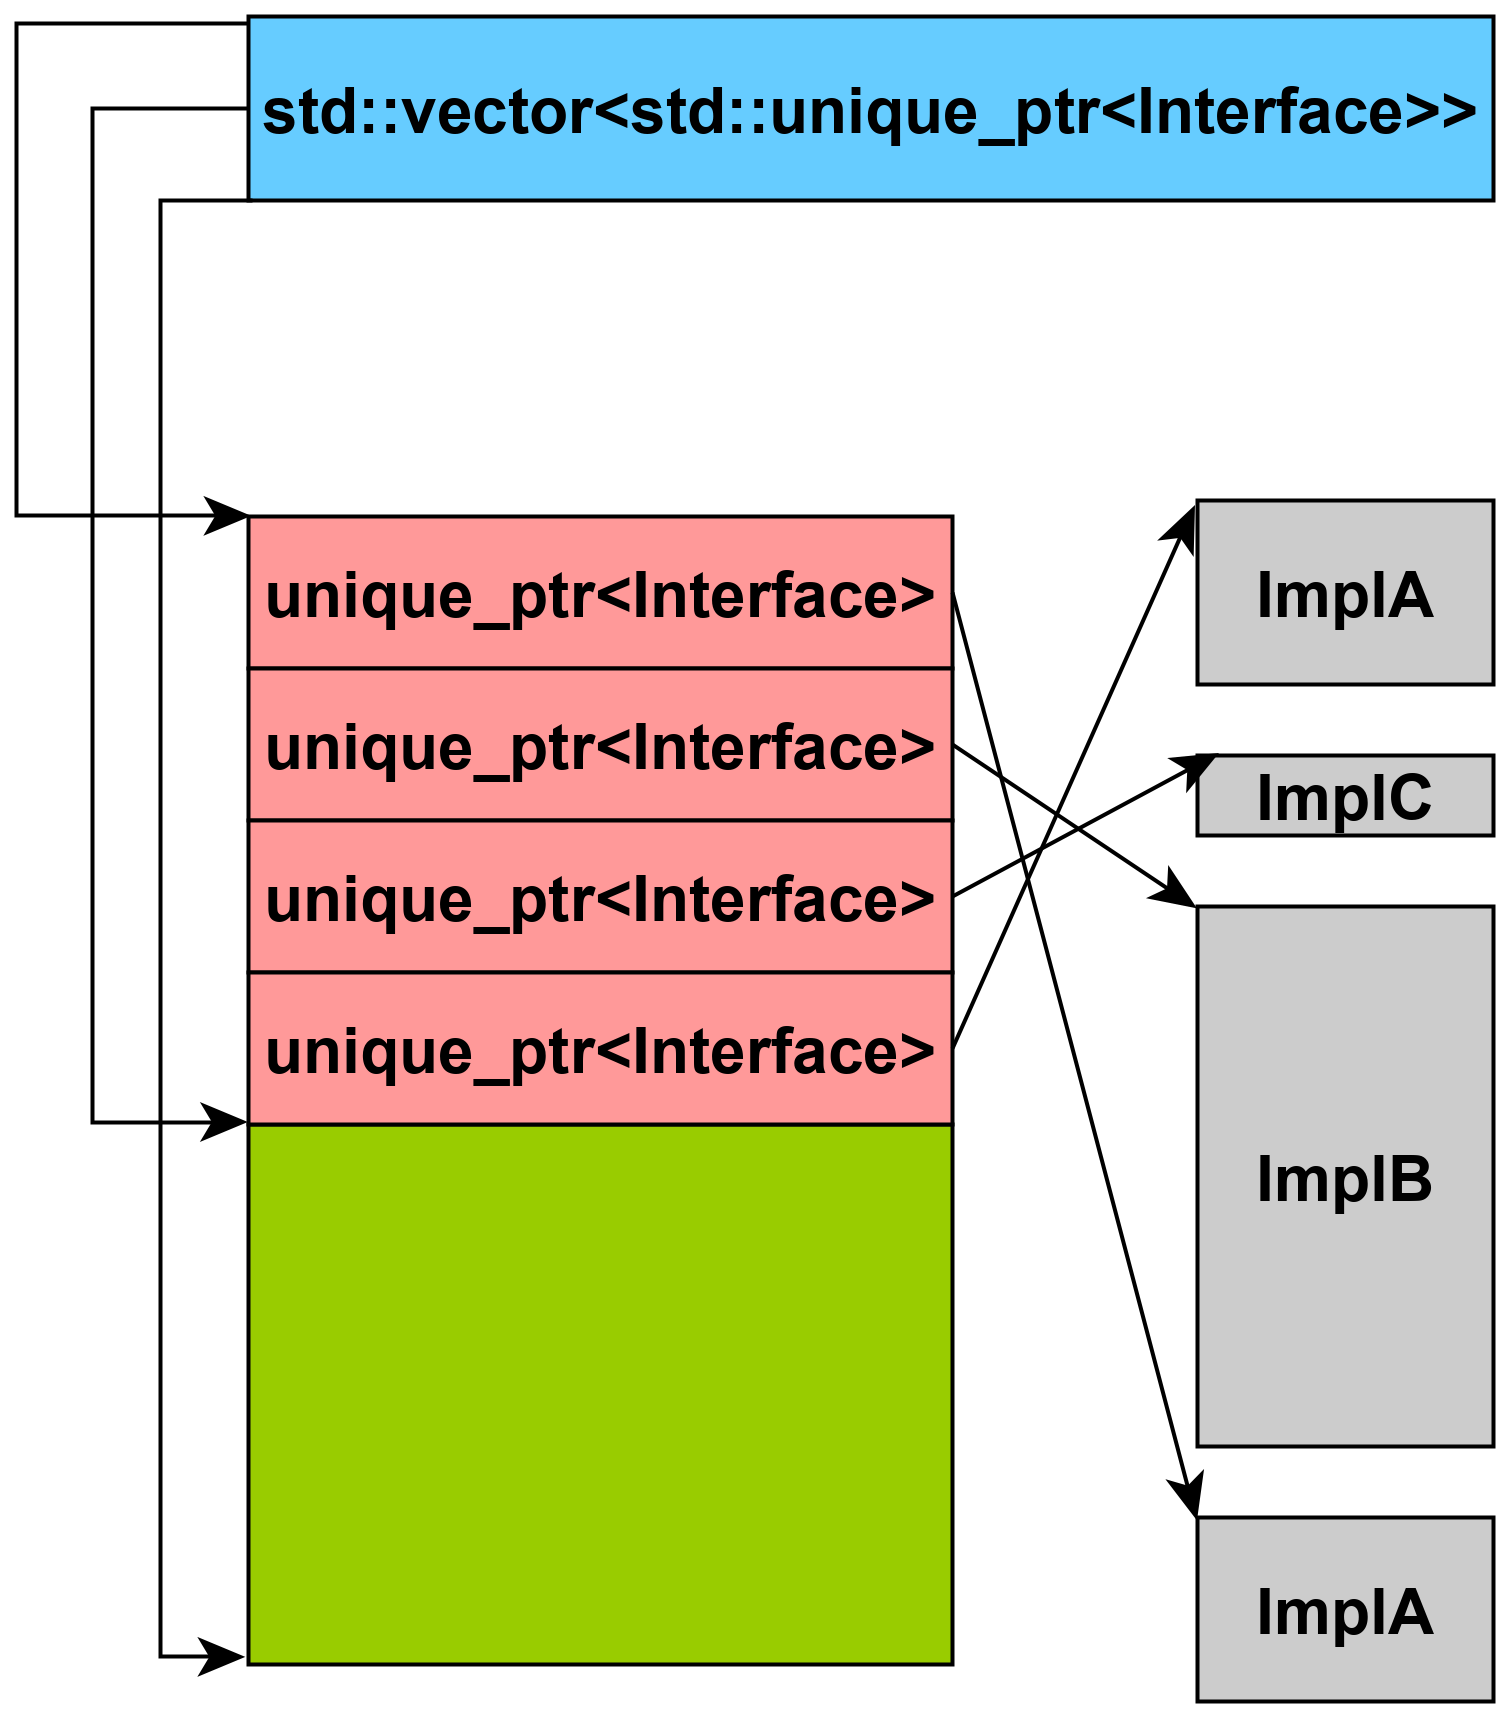
\includegraphics[width=0.9\linewidth]{std_vec.png}
    \caption{A possible memory layout when \lstinline{std::vector<std::unique_ptr<Interface>>} is used}
    \label{fig:stdvecbased}
\end{minipage}%
\begin{minipage}{.5\textwidth}
    \centering
    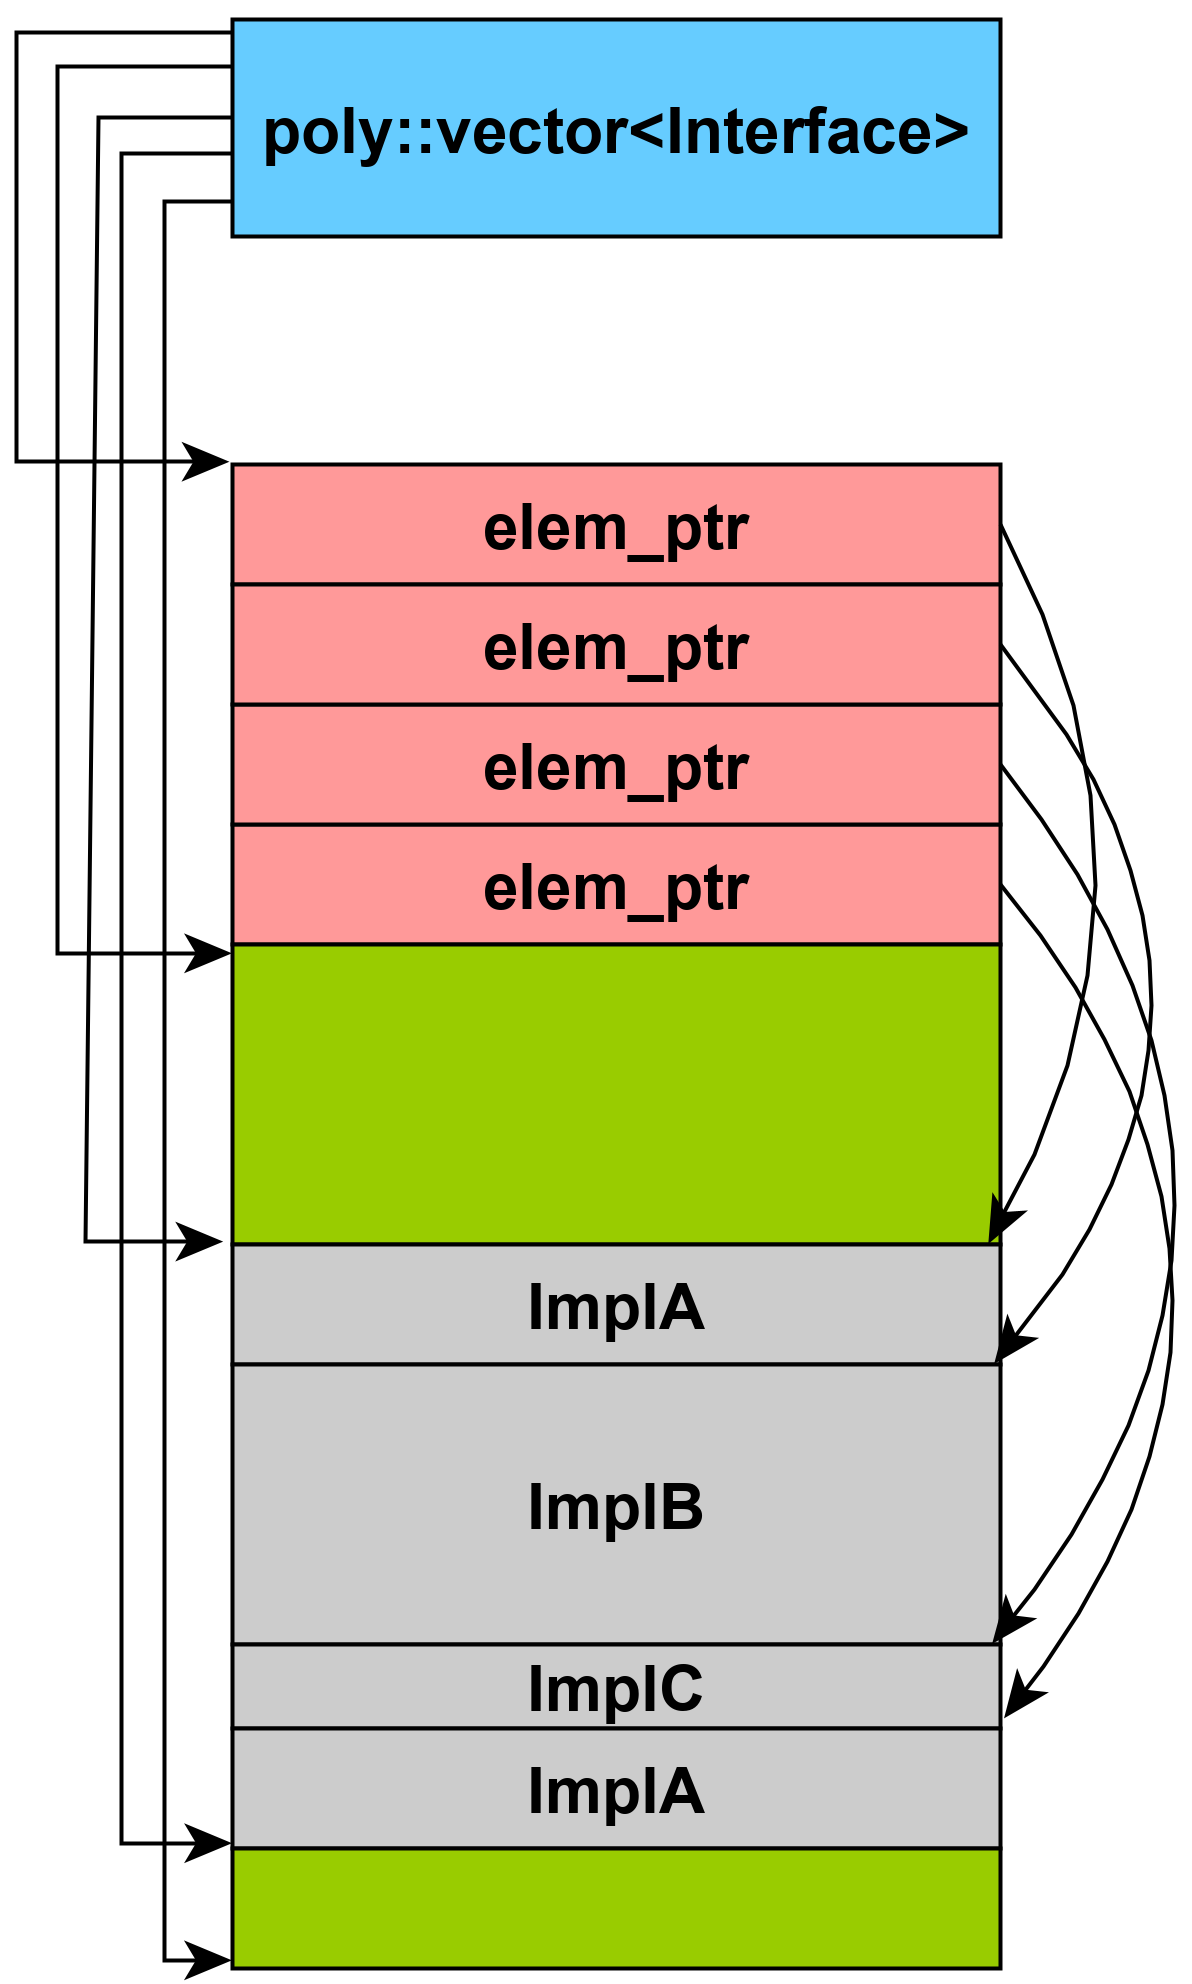
\includegraphics[width=0.75\linewidth]{poly_vec_fig.png}
    \caption{Guaranteed layout when \lstinline{poly::vector<Interface>} is used}
    \label{fig:polyvecbased}
\end{minipage}
\end{figure}

\newpage

\section{Design}

While STL already presents a solution for dynamic memory management abstraction in the form of \emph{Allocators} - an application of policy-based class design \cite{alexandrescu_2011_policybasedclassdesign} - the key for managing/storing objects in this fashion is cloning/moving. For addressing the other problem of relocating objects through their interface reference, another concept has to be introduced in the form of a \emph{CloningPolicy}. This can be described as a concept, as seen on Listing \ref{lst:cloningpolicyconcept}. 

%TODO: add c++20 concepts definitions for cloning policy here).

\begin{lstlisting}[label={lst:cloningpolicyconcept},caption={CloningPolicy concept definition},captionpos=b]
namespace poly 
{
template <typename T> 
struct type_tag 
{
  using type = T;
};
} //namespace poly 
using namespace poly;
using namespace std;

template <typename InterfaceT, typename Allocator>
constexpr auto AllocatorPointerMatch = is_same_v<InterfaceT,
  typename pointer_traits<
    typename allocator_traits<Allocator>::pointer>::element_type>;

template <typename T, typename InterfaceT, typename Allocator>
concept HasClone = requires(T cp, Allocator a)
  {
    {
      cp.clone(a, declval<typename allocator_traits<Allocator>::pointer>(),
        declval<typename allocator_traits<Allocator>::void_pointer>())
    } -> same_as<typename allocator_traits<Allocator>::pointer>;
  };

template <typename T, typename InterfaceT, typename Allocator>
concept HasMove  = 
  is_nothrow_move_constructible_v<T> && 
  is_nothrow_move_assignable_v<T> && 
  requires(T cp, Allocator a)
  {
    {
      cp.move(a, declval<typename allocator_traits<Allocator>::pointer>(),
        declval<typename allocator_traits<Allocator>::void_pointer>())
    } -> same_as<typename allocator_traits<Allocator>::pointer>;
  };

template <typename T, typename I, typename A, typename Derived>
concept CloningPolicy = 
  AllocatorPointerMatch<I, A> &&
  is_nothrow_constructible_v<T> &&
  is_nothrow_copy_constructible_v<T> &&
  is_nothrow_copy_assignable_v<T> &&
  copyable<T> && 
  (constructible_from<T, type_tag<Derived>> || default_initializable<T>) &&
  (HasClone<T, I, A> || HasMove<T, I, A>);

\end{lstlisting}

The cloning policy must be able to clone - move if supported - objects around in memory through a base class pointer. The new additions to the typical class hierarchy are emphasized using the green color in Figure \ref{fig:polyvecdesign}. The other component is the element pointer, which can be thought of as a decentralized smart pointer as the smart pointer operation is realized by two collaborating classes really: the vector and the element pointer itself as the vector is managing the lifetime while the access is provided through the element pointer. 

\begin{figure}[!htb]
    \centering
    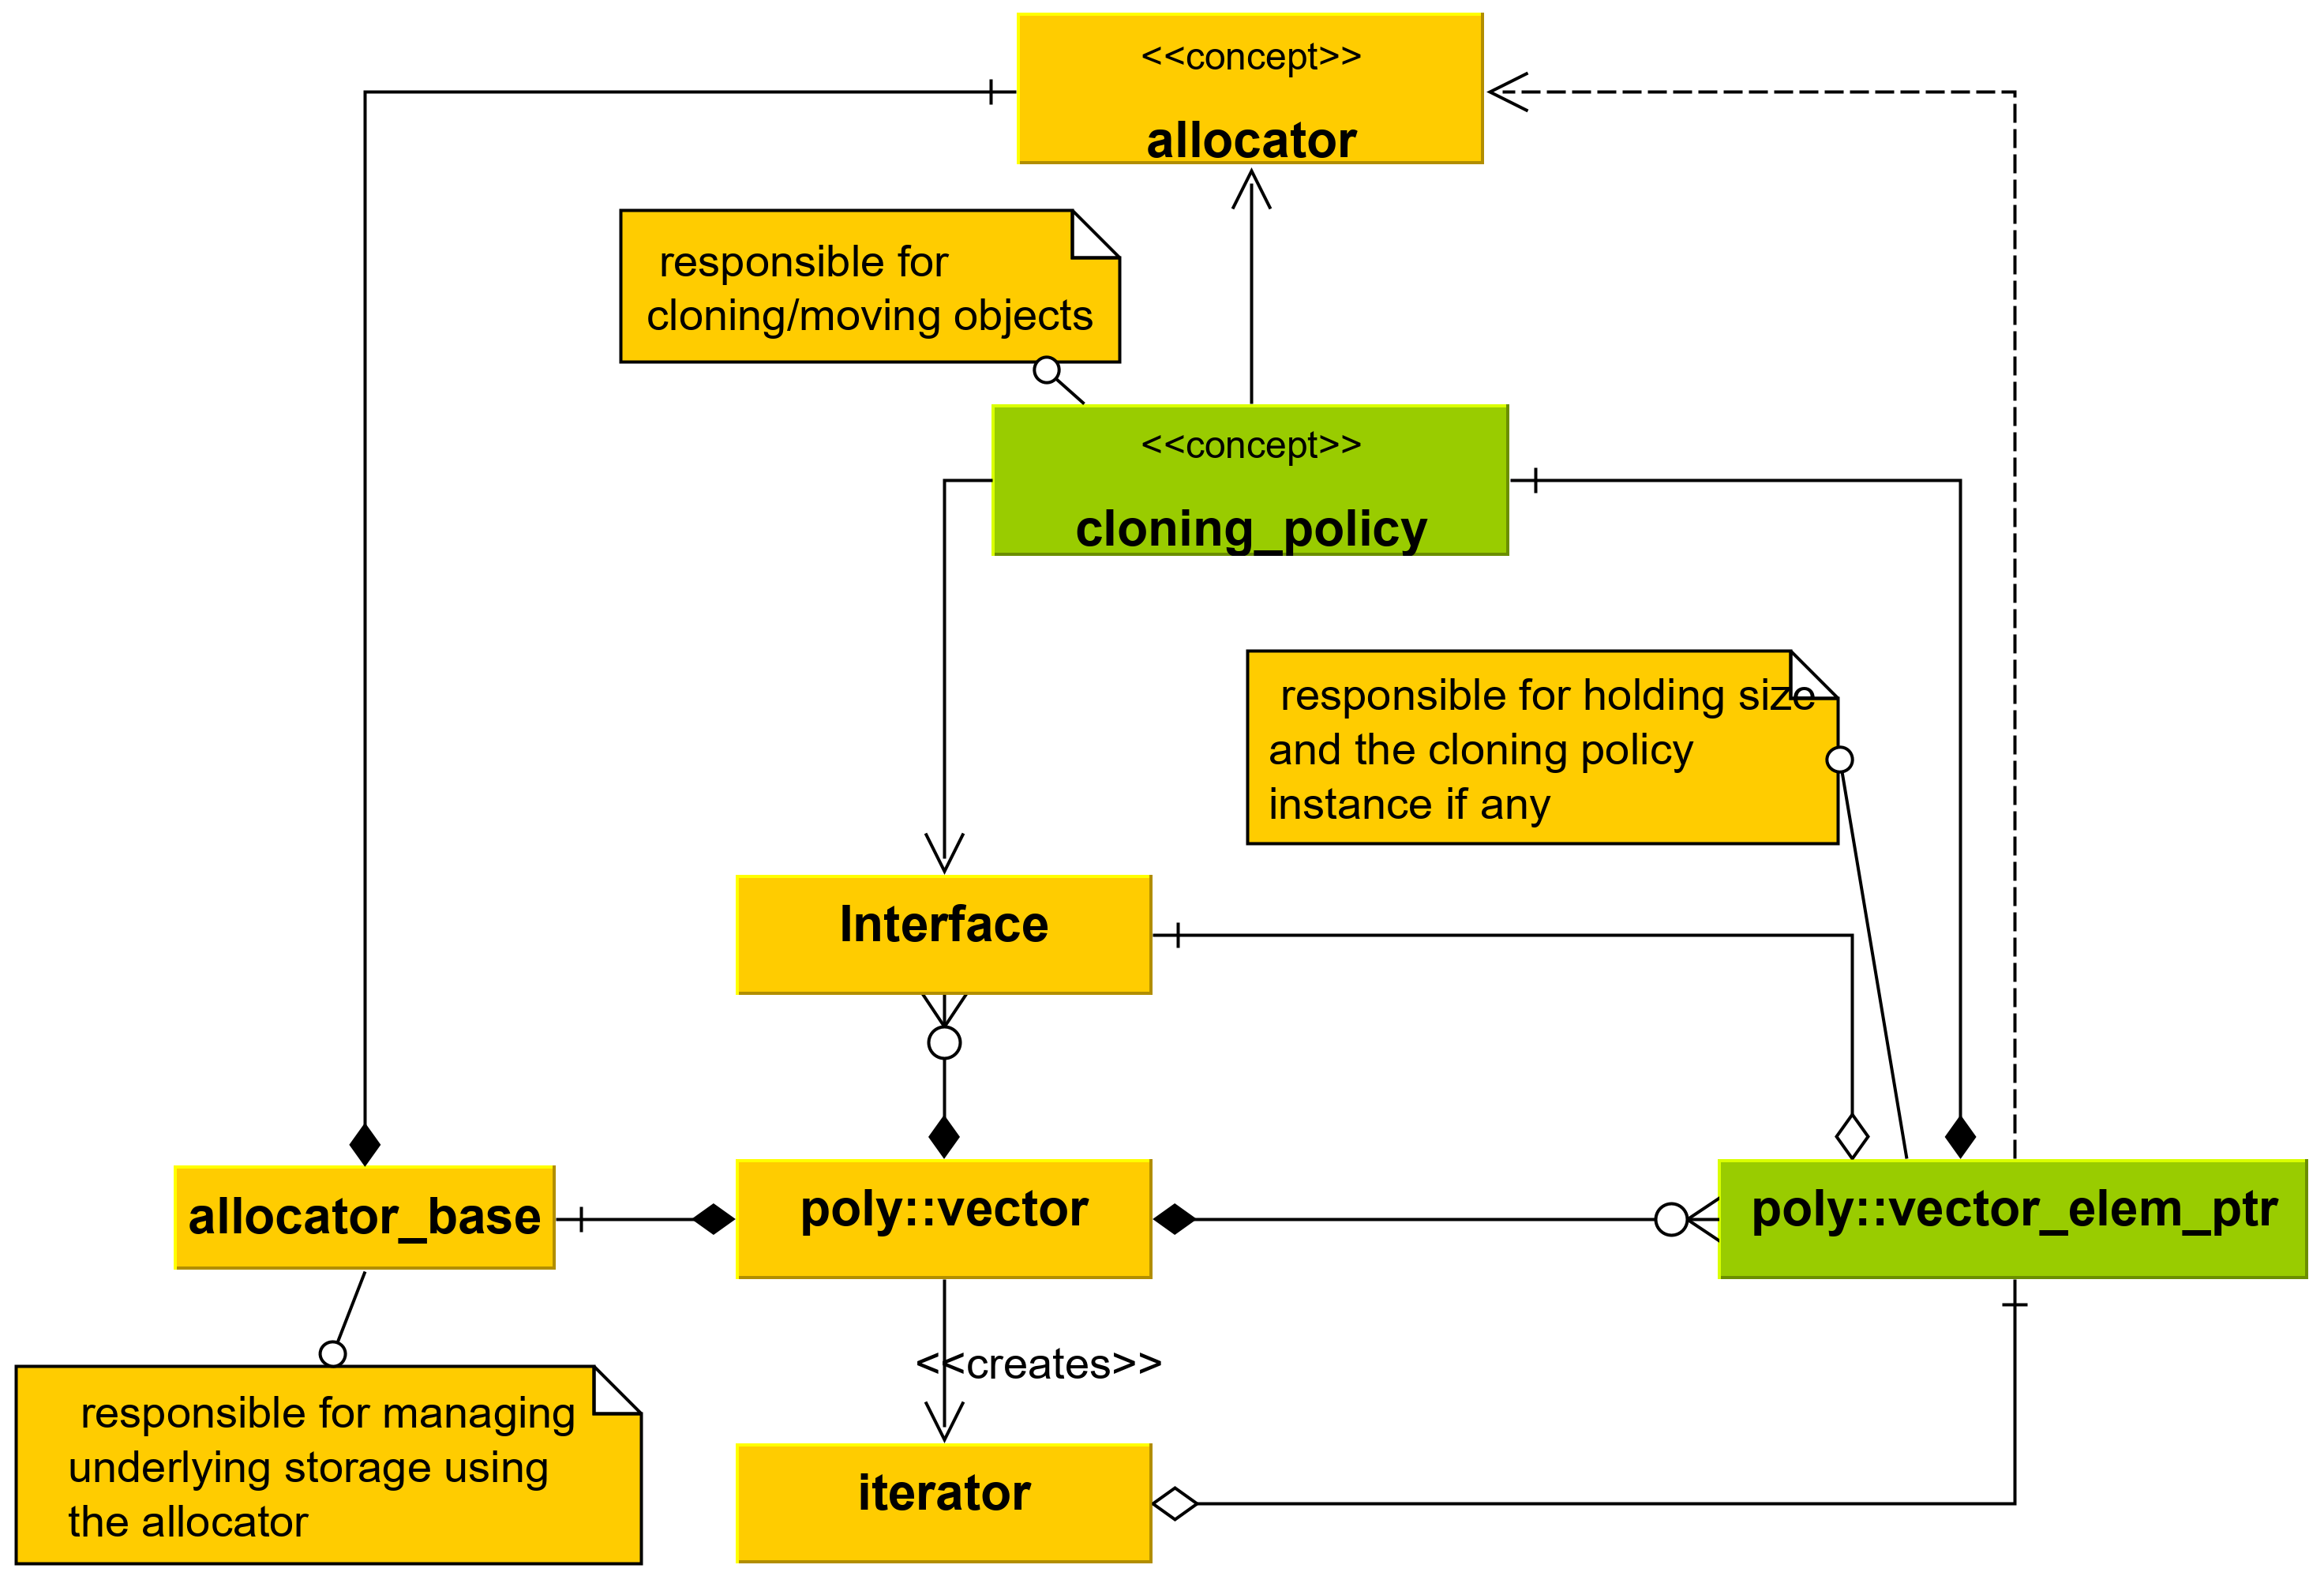
\includegraphics[width=0.95\textwidth]{polyvecdesign.png}
    \caption{The UML class diagram of the components of \lstinline{poly::vector<T>} (NB.: UML elements for indicating class templates were deliberately left out)}
    \label{fig:polyvecdesign}
\end{figure}

Two archetypes of cloning policies have been designed: \lstinline{delegate_cloning_policy} and \lstinline{no_cloning_policy}. The former is suitable for the most common use cases where the derived classes are regular in terms of copy/move. As one might assume, this cloning policy captures the way of cloning/moving at the time of insertion to the container. That also means the static type of the object inserted must be known at compile time at the point of insertion. The latter does not allow any copy/move of an object, i.e.,  if the container capacity is exhausted, then a \lstinline{std::bad_alloc} exception is raised.

Since \lstinline{cloning_policy} is a concept - as denoted in Figure \ref{fig:polyvecdesign} - the user can supply a type that suits the actual class hierarchy whose instances are stored in the container. For example, if there is already a \emph{Clone} virtual member function declared in the interface, a policy class can be written quickly to use that function when the container must copy the objects to a new location, e.g., because of a resize.


The classic \emph{size} and \emph{capacity} concept has to be augmented in this container: here, an average size is considered as \emph{size}, which is the total amount of memory occupied by the objects stored in the container divided by the number of objects. The container's exponential growth  is also performed based on the average size (including the to-be inserted the element in the average).

Besides these, the aim was to provide the same level of exception safety and API as one would expect from the \lstinline{std::vector<std::unique_ptr<Interface>>} based implementation.


\section{Evaluation and Measurements}

Time-based measurements are not trivial to carry out during software-benchmarking  and when using a non-realtime OS. For these scenarios, the measurement metric is the overall execution wall clock time. This is provided by the OS through a high resolution clock - for specific operations over a given object count that is processed through the containers \cite{Measuring_Throughput}. For the evaluation, a demo \emph{Interface} class has been defined with two distinct and different sized implementation classes. The vectors under test were populated randomly from these two types. To minimize the variance of the measurements, the concept of static thread affinity (a.k.a thread pinning) was used hand-in-hand with setting the highest priority (smallest \emph{nice} value) for the benchmark process. This way, the process will not be scheduled away that much, and most of the cache trashing occurs because of the benchmark program itself and not by the rescheduling. 


The evaluation of the container was based on three sets of measurement scenarios that have been defined as the following:
\begin{itemize}
    \item total number of allocation count, that is, how many times  did the program allocate memory from the runtime environment - the smaller value is the better;
    \item best-case scenario, when the objects are populated into the vector in a successive manner without any in-between allocations from other places, benchmark the sequential access time - smaller value is better;
    \item worst-case scenario, when the objects are populated into the vector where in-between allocations happen from other places resulting in each and every object being on a separate page, benchmark the sequential access time - smaller value is better (NB.: this is simply emulated by allocating a page for an object and constructing it there).
\end{itemize}

\begin{figure}[!htb]
    \centering
    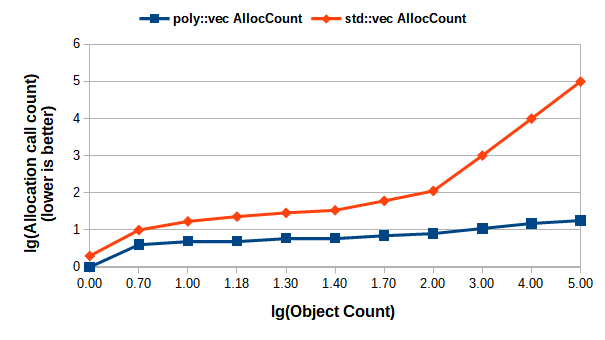
\includegraphics[width=0.95\textwidth]{alloccount-meas.png}
    \caption{Measurement result of total allocation count (including object allocation managed by smart pointers)}
    \label{fig:meas-alloccount}
\end{figure}
\begin{figure}[!htb]
    \centering
    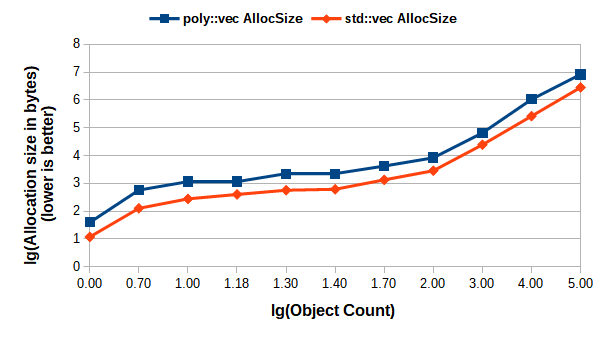
\includegraphics[width=0.95\textwidth]{allocsize-meas.png}
    \caption{Measurement result of total allocation size (including object allocation managed by smart pointers)}
    \label{fig:meas-allocsize}
\end{figure}

Figure \ref{fig:meas-alloccount} shows the total allocation count, while Figure \ref{fig:meas-allocsize} the allocated size of memory, including the allocations made as a result of storing the object on heap managed by a smart pointer handle.  The data has been plotted using a log-log scale for better clarity. 
Figure \ref{fig:meas-alloccount} and Figure \ref{fig:meas-allocsize} should be interpreted together, e.g., for 1000 objects  (at coordinate three on the horizontal axis) of randomly chosen types from the demo class hierarchy, there were a total of 11 calls to the allocator's allocate member function with the total size of 66006 bytes, while for the std::vec alternative the total allocation calls were 1018 with the total size of 24812 bytes - on average. 
As one can see, the total allocation count is smaller for \lstinline{poly::vector}, which is a consequence of the omitted heap allocation when the objects are instantiated, while the total size is slightly greater for \lstinline{poly::vector}. This is because  that \lstinline{poly::vector} is growing its capacity exponentially -- based on the average size that is a weighted average of all stored objects size. This trade-off for ensuring the locality incurs somewhat higher memory utilization. However, the benefit of reduced allocation count is obvious. Furthermore, it is even more significant when allocators from the \emph{pmr} namespace  are used, as the \emph{allocate} call there will not be inlined normally - without devirtualization, as it is a dynamically dispatched call. This adds more penalty if there are more allocations made than necessary.


\begin{figure}[!htb]
    \centering
    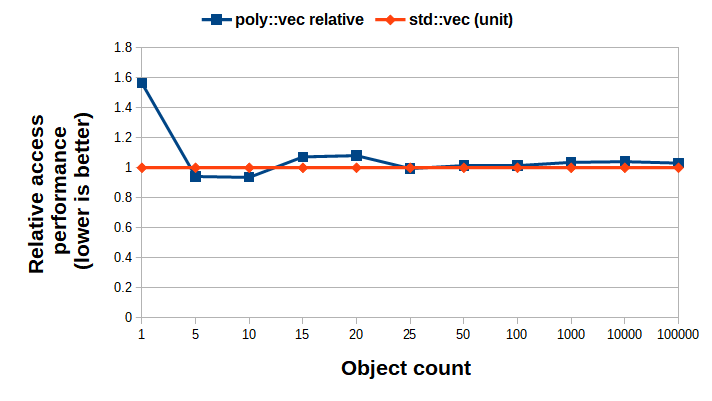
\includegraphics[width=0.95\textwidth]{acces-bc-meas.png}
    \caption{Measurement result of best-case scenario access performance}
    \label{fig:meas-access-bc}
\end{figure}
\begin{figure}[!htb]
    \centering
    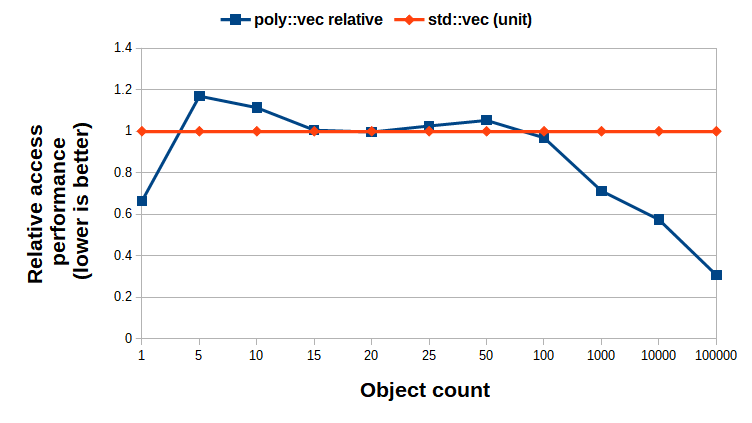
\includegraphics[width=0.95\textwidth]{acces-wc-meas.png}
    \caption{Measurement result of worst-case scenario access performance}
    \label{fig:meas-access-wc}
\end{figure}

The measurement data that was used to generate Figure \ref{fig:meas-access-bc} and Figure \ref{fig:meas-access-wc} is based on average values. Multiple measurements were carried out for the same object count, and the statistical difference was determined by using two-tail Student T-test with unequal variances, $\alpha = 0.01$. For Figure \ref{fig:meas-access-bc} - that shows the averages for the best-case scenario - based on the raw data at the key points, there is no statistical significance of the differences between the averages. Therefore we can say that most probably \lstinline{poly::vector} is not worse than the \lstinline{std::vector} based alternative in this aspect. In the worst-case scenario - illustrated by Figure \ref{fig:meas-access-wc} - the raw data showed that until the object count reaches 100, the difference is statistically insignificant, and also showed that for greater object count, \lstinline{poly::vector} outperforms the STL based alternative in terms of sequential access performance. (NB.: For the small object count measurements, the variance was so significant and also the timings were inaccurate that no real consequence can be deduced from those data points).

Another important aspect - yet less tangible in terms of performance - is the syntactic verbosity of \lstinline{poly::vector} compared to the \lstinline{std::vector}. Even though it has no runtime impact, it is still much more convenient to express ideas directly in code. As an example: if the programmer wishes to place an object of polymorphic type into a container, currently a smart pointer has to be created, memory to be allocated, the object to be constructed and assigned to the smart pointer handle instance for memory and lifetime management, then inserted into the container itself. With \lstinline{poly::vector}, this is not the case: the intention is expressed directly. This argument is analogous to the \lstinline{for} loop versus STL range-based algorithms. While each has its place, the intention and the business logic are still more clearly communicated using the latter.


\section{Conclusion}
In this paper, a generic container has been described that is tailored for storing polymorphic instances derived from a well-known interface. Due to the underlying memory and layout management, locality of references is enforced structurally, which results in increased sequential access performance with greater object counts, while also reducing the total number of allocation count which could also be beneficial from performance perspective. The trade-off for achieving this is an increased memory utilization, as the container maintains capacity not just for the \emph{objects handles} but also for the yet to be stored objects based on an average size computation. It has also been shown that with the best-case allocation scheme the access performance is comparable to the standard based alternative. 

In summary this container can be used as a drop in replacement for \lstinline{std::vector<std::unique_ptr<InterfaceType>>} pattern in high performance applications that use OOP for abstraction but still want to eliminate the penalties due to memory fragmentation. 

\bibliographystyle{plain}
\bibliography{references}


\end{document}